% IN5450 Project 1 – Array Signal Processing
% Build: pdflatex -interaction=nonstopmode -halt-on-error presentation_p1.tex

\documentclass[aspectratio=169,9pt]{beamer}

\usetheme{Madrid}
\usecolortheme{default}

\usepackage{graphicx}
\usepackage{amsmath,amssymb}
\usepackage{booktabs}
\usepackage{mathtools}
\usepackage[T1]{fontenc}
\usepackage[utf8]{inputenc}
\usepackage{listings}

\graphicspath{{figs/}}

\setbeamertemplate{footline}[frame number]
\setbeamertemplate{navigation symbols}{}

% Tighter vertical spacing
\setlength{\parskip}{2pt plus 1pt}

% Figure helpers
\newcommand{\fullfig}[2][]{%
  \centering
  \includegraphics[width=\linewidth,height=0.75\textheight,keepaspectratio,#1]{#2}%
}
\newcommand{\colfig}[2][]{%
  \includegraphics[width=\linewidth,height=0.55\textheight,keepaspectratio,#1]{#2}%
}

% Listing style for MATLAB
\lstset{
  language=Matlab,
  basicstyle=\ttfamily\fontsize{5.5pt}{6.5pt}\selectfont,
  keywordstyle=\color{blue}\bfseries,
  commentstyle=\color{green!50!black},
  stringstyle=\color{red!70!black},
  breaklines=true,
  frame=single,
  numbers=none,
  columns=flexible
}

\title[IN5450 Project 1]{Diffraction \& Array Patterns\\IN5450 Project 1}
\author{Theodor W\aa lberg}
\institute{University of Oslo}
\date{March 2026}

\begin{document}

% ----
\begin{frame}
  \titlepage
\end{frame}

% ----
\begin{frame}{Agenda}
  \tableofcontents
\end{frame}

% ==================================================================
\section{Diffraction from a Line Aperture (Tasks 1-2)}
% ==================================================================

% -- SLIDE: Task 1 --
\begin{frame}{Task 1 - Diffraction field of a line aperture}
\vspace{-0.3em}
\textbf{Setup:} Uniform line aperture $D=20\lambda$, $f_0=3$\,MHz, $c=1500$\,m/s.
R-S integral evaluated via \texttt{R\_S\_LinAperture.m}.

\begin{columns}[T]
\column{0.48\textwidth}
\colfig{image-21.png}
\smallskip
\scriptsize \textbf{Near-field} ($r\approx z_R$): Irregular amplitude with ripples
due to path-length interference from different parts of the aperture.
\column{0.48\textwidth}
\colfig{farfield.png}
\smallskip
\scriptsize \textbf{Far-field} ($r\gg z_R$): Smooth $\mathrm{sinc}$-like pattern -
field $\propto$ spatial FT of aperture distribution.
\end{columns}

\smallskip
\scriptsize Transition from near-field to far-field is clearly visible in the increasing smoothness of the angular response.
\end{frame}

% -- SLIDE: Code 1-2 --
\begin{frame}[fragile]{Code - Diffraction \& \texttt{beampattern.m}}
\vspace{-0.3em}
\begin{columns}[T]
\column{0.48\textwidth}
\scriptsize\textbf{Core utility (used in all tasks):}
\begin{lstlisting}
function W = beampattern(xpos, kx, weights)
  xpos = xpos(:); weights = weights(:); kx = kx(:);
  W = exp(1j*kx.*xpos.') * weights;
end
\end{lstlisting}

\smallskip
\scriptsize\textbf{R-S diffraction setup (Tasks 1-2):}
\begin{lstlisting}
D = 20*lambda;  dx = lambda/10;
apX = -D/2:dx:D/2;
A0 = ones(size(apX)).'; A0 = A0/sum(A0);
z_R = D^2 / (4*lambda);

% 2D field
[Resp2D, ~] = R_S_LinAperture(apX, apZ, ...
                               X, Z, lambda, A0);
\end{lstlisting}

\column{0.48\textwidth}
\scriptsize\textbf{Half-circle at near-/far-field:}
\begin{lstlisting}
us = -pi/2:du:pi/2;
% Near-field half-circle at r = z_R
Z_near = z_R*cos(us);
X_near = z_R*sin(us);
[Resp_near, ~] = R_S_LinAperture(apX, apZ,...
                  X_near, Z_near, lambda, A0);

% Far-field half-circle at r = 10*z_R
r_far = 10*z_R;
Z_far = r_far*cos(us);
X_far = r_far*sin(us);
[Resp_far, ~] = R_S_LinAperture(apX, apZ,...
                  X_far, Z_far, lambda, A0);
\end{lstlisting}
\end{columns}
\end{frame}

% -- SLIDE: Task 2 --
\begin{frame}{Task 2 - 2D field \& near-/far-field boundary}
\vspace{-0.5em}
\begin{columns}[T]
\column{0.48\textwidth}
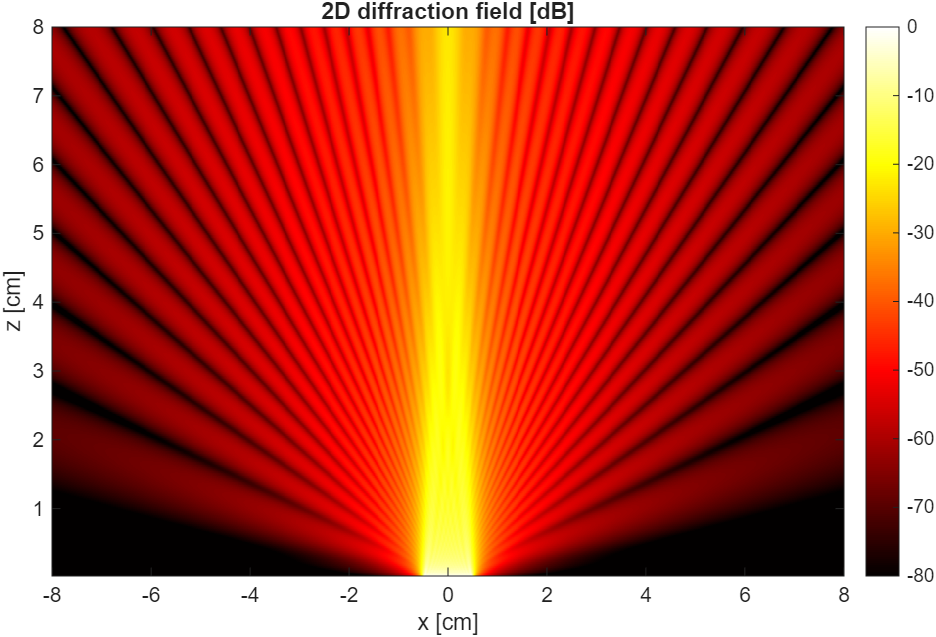
\includegraphics[width=\linewidth,height=0.22\textheight,keepaspectratio]{image-24.png}\\[-2pt]
{\scriptsize 2D field: beam confined near aperture, spreading at larger $z$.}

\smallskip
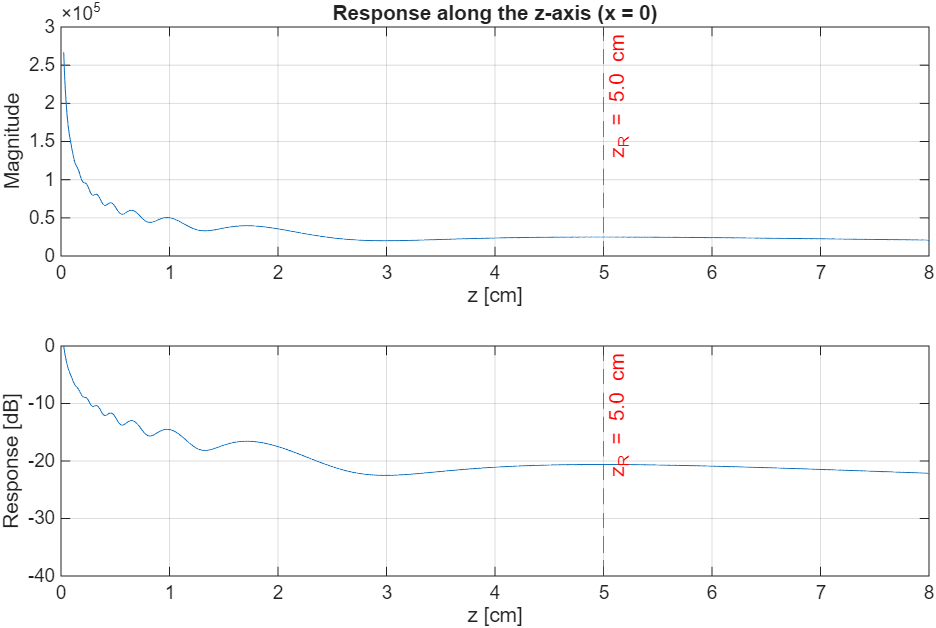
\includegraphics[width=\linewidth,height=0.22\textheight,keepaspectratio]{image-23.png}\\[-2pt]
{\scriptsize On-axis: amplitude oscillates in NF, decays as $1/\!\sqrt{z}$ beyond $z_R$.}

\smallskip
%% TODO: uncomment when image-23-norm.png is exported from MATLAB figure(2) subplot 3
%\includegraphics[width=\linewidth,height=0.22\textheight,keepaspectratio]{image-23-norm.png}\\[-2pt]
%{\scriptsize Normalised (corrected for $1/\!\sqrt{r}$): converges to constant beyond $z_R$.}
\column{0.48\textwidth}
\scriptsize
\textbf{Derivation:}
$$\Delta\phi_\text{max} = \frac{\pi D^2}{4\lambda z}$$

\vspace{-0.6em}
Setting $\Delta\phi_\text{max}=\pi/2$ (path diff.\ $=\lambda/4$):
$$\boxed{z_R = \frac{D^2}{4\lambda}} = 100\lambda = 5\text{\,cm}$$

\vspace{-0.3em}
\scriptsize Differs from piston formula $2D^2/\lambda$ which uses a stricter phase criterion for 2D apertures.

\medskip
\textbf{At $r\!=\!z_R$:} NF artifacts; sidelobes not stabilised.\\[1pt]
\textbf{At $r\!=\!10z_R$:} Smooth sinc, first SL $=-13.2$\,dB.

\medskip
\textbf{Normalised response:} After correcting for $1/\!\sqrt{r}$ spreading, the on-axis response converges to a constant beyond $z_R$, providing a visual alternative NF/FF limit.

\medskip
{\fontsize{4.5pt}{5.5pt}\selectfont \textbf{Ref:} S.~Holm, \emph{IN5450 Diffraction: from waves to signal processing}, UiO, 2019.}
\end{columns}
\end{frame}

% ==================================================================
\section{Grating Lobes (Task 4)}
% ==================================================================

% -- SLIDE: Task 4 --
\begin{frame}{Task 4 - Effect of element spacing on grating lobes}
\vspace{-0.3em}
\textbf{Setup:} $M=24$ ULA, unity weights, $d = \lambda/4,\;\lambda/2,\;\lambda,\;2\lambda$.

\vspace{-0.3em}
\fullfig{image-6.png}

\vspace{-0.5em}
\scriptsize
\begin{itemize}\setlength\itemsep{0pt}
  \item $d=\lambda/4$: Wide main lobe ($8.5^\circ$), no grating lobes; small aperture gives poor resolution.
  \item $d=\lambda/2$: BW $\approx4.2^\circ$, max SL $=-13.2$\,dB. No grating lobes gives good balance.
  \item $d=\lambda$: Grating lobe at $u=\pm1$ ($\theta=\pm90^\circ$). Spatial Nyquist violated.
  \item $d=2\lambda$: Multiple grating lobes at $\Delta u = \lambda/d = 0.5$. Ambiguous direction finding.
\end{itemize}
\end{frame}

% -- SLIDE: Code 4 --
\begin{frame}[fragile]{Code - Grating lobe analysis (Task 4)}
\vspace{-0.3em}
\begin{lstlisting}
M = 24;  weights = ones(M,1)/M;
spacings = [1/4, 1/2, 1, 2];   % in units of lambda
u = linspace(-1, 1, 10000);  kx = 2*pi/lambda * u;

for i = 1:4
    d    = spacings(i) * lambda;
    xpos = (0:M-1).' * d;           % ULA positions
    W    = beampattern(xpos, kx, weights);

    Result = analyzeBP(u, W);
end
\end{lstlisting}

\smallskip
\scriptsize
\texttt{analyzeBP} returns beamwidths (at $-3$\,dB and $-6$\,dB) and maximum sidelobe level.
Grating lobes appear when $d \ge \lambda$ since the beampattern is periodic with $\Delta u = \lambda/d$.
\end{frame}

% ==================================================================
\section{Kaiser Window (Task 5)}
% ==================================================================

% -- SLIDE: Task 5 figure --
\begin{frame}{Task 5 - Kaiser window on $M=24$, $d=\lambda/2$}
\vspace{-0.3em}
\textbf{Setup:} Kaiser window $\beta=0\text{-}5$. Report beamwidths, max SL, WNG.

\vspace{-0.3em}
\fullfig{image-7.png}

\vspace{-0.3em}
\scriptsize WNG $= |\sum w_m|^2/\sum|w_m|^2$. Uniform weighting maximises WNG at $10\log_{10}(24)=13.8$\,dB.
\end{frame}

% -- SLIDE: Task 5 table --
\begin{frame}{Task 5 - Results}
\vspace{-0.3em}
\scriptsize
\begin{tabular}{ccccc}
\toprule
$\beta$ & $-3$\,dB BW ($^\circ$) & $-6$\,dB BW ($^\circ$) & Max SL (dB) & WNG (dB) \\
\midrule
0.0 & 4.21 & 5.74 & $-13.2$ & 13.8 \\
1.0 & 4.37 & 5.97 & $-14.7$ & 13.8 \\
2.0 & 4.78 & 6.57 & $-19.0$ & 13.6 \\
3.0 & 5.33 & 7.35 & $-25.0$ & 13.2 \\
4.0 & 5.88 & 8.18 & $-31.7$ & 12.7 \\
5.0 & 6.43 & 8.96 & $-38.0$ & 12.3 \\
\bottomrule
\end{tabular}

\medskip
\normalsize
\begin{itemize}\setlength\itemsep{1pt}
  \item \textbf{Advantage:} SL drops from $-13$ to $-38$\,dB - critical for rejecting interferers.
  \item \textbf{Disadvantage:} Main lobe broadens ($4.2^\circ\to6.4^\circ$); WNG drops slightly ($13.8\to12.3$\,dB).
  \item Each ${\sim}12$\,dB of SL suppression costs ${\sim}1^\circ$ of mainlobe broadening.
\end{itemize}
\end{frame}

% -- SLIDE: Code 5 --
\begin{frame}[fragile]{Code - Kaiser window \& WNG (Task 5)}
\vspace{-0.3em}
\begin{lstlisting}
d = lambda/2;  xpos = (0:M-1).' * d;
betas = 0:0.5:5;

for i = 1:length(betas)
    w = kaiser(M, betas(i));    % Kaiser window
    w = w / sum(w);             % normalise so sum(w) = 1

    W = beampattern(xpos, kx, w);

    % White noise gain: WNG = |sum(w)|^2 / sum(|w|^2)
    % Since sum(w) = 1:  WNG = 1 / sum(w.^2)
    WNG = 1 / sum(w.^2);

    Result = analyzeBP(u, W);
end
\end{lstlisting}

\smallskip
\scriptsize
Higher $\beta$ concentrates weight energy in fewer elements $\Rightarrow$ SL drops but BW broadens.
WNG penalises non-uniform weights: $\mathrm{WNG} = |\sum w_m|^2 / \sum|w_m|^2$.
\end{frame}

% ==================================================================
\section{Non-uniform Spacing (Task 6)}
% ==================================================================

% -- SLIDE: Task 6 --
\begin{frame}{Task 6 - Uniform vs.\ Kaiser vs.\ Case B}
\vspace{-0.5em}
\begin{columns}[T]
\column{0.55\textwidth}
\colfig{image-8.png}
\column{0.44\textwidth}
\scriptsize
\begin{tabular}{lccc}
\toprule
Array & WNG & $-3$\,dB & Max SL \\
\midrule
Uniform & 13.8 & $4.21^\circ$ & $-13.2$ \\
Kaiser $\beta\!=\!3$ & 13.2 & $5.33^\circ$ & $-25.0$ \\
Case B & 13.8 & $4.55^\circ$ & $-17.9$ \\
\bottomrule
\end{tabular}

\smallskip\normalsize
Case B uses uniform weights and achieves full WNG, but element positions are optimised to reduce SL. BW is slightly wider than uniform but much narrower than Kaiser.

\smallskip
$\approx 5$\,dB SL improvement over uniform with only $0.3^\circ$ BW cost.

\smallskip
Optimising element positions reduces SL without sacrificing noise robustness.
\end{columns}
\end{frame}

% ==================================================================
\section{Steering (Tasks 7-8)}
% ==================================================================

% -- SLIDE: Task 7 --
\begin{frame}{Task 7 - Steering the Case B array}
\vspace{-0.3em}
\begin{columns}[T]
\column{0.48\textwidth}
\textbf{Unsteered, $u\in[-2,2]$:}
\colfig{image-9.png}
\scriptsize Outside the visible region the beampattern continues. When steered, this structure can enter the visible region.
\column{0.48\textwidth}
\textbf{Steered} ($\theta_s = 0^\circ,20^\circ,40^\circ,60^\circ$):
\colfig{image-10.png}
\scriptsize Main lobe broadens and SLs grow at large steering angles.
\end{columns}
\end{frame}

% -- SLIDE: Task 8 --
\begin{frame}{Task 8 - Beamwidth vs.\ steering angle (Case B)}
\vspace{-0.3em}
\fullfig{image-11.png}

\vspace{-0.3em}
\scriptsize
\textbf{Result:} BW in degrees increases with steering angle ($\propto 1/\cos\theta_s$),
but BW in $\sin\theta$ (computed as $\sin\theta_R - \sin\theta_L$) remains approximately constant --- the broadening is a purely geometric projection effect.
\end{frame}

% ==================================================================
\section{Thinned Arrays (Task 9)}
% ==================================================================

% -- SLIDE: Task 9 overlays --
\begin{frame}{Task 9 - Random thinning (200 realisations)}
\vspace{-0.3em}
\textbf{Setup:} $M=101$, $d=\lambda/2$. Randomly select $N$ elements (outer two fixed).

\begin{columns}[T]
\column{0.32\textwidth}
\colfig{image-12.png}
\centering\scriptsize $N=25$
\column{0.32\textwidth}
\colfig{image-13.png}
\centering\scriptsize $N=50$
\column{0.32\textwidth}
\colfig{image-14.png}
\centering\scriptsize $N=75$
\end{columns}

\smallskip
\scriptsize Red = dense $N\!=\!101$ reference. Grey spread narrows as $N$ increases; SL floor converges to dense array.
\end{frame}

% -- SLIDE: Task 9 stats --
\begin{frame}{Task 9 - Thinning statistics \& optimal arrays}
\vspace{-0.5em}
\begin{columns}[T]
\column{0.54\textwidth}
\scriptsize
\textbf{Random thinning:}\\[2pt]
\begin{tabular}{lcccc}
\toprule
$N$ & BW ($^\circ$) & $\sigma_\text{BW}$ & Max SL & Mean SL \\
\midrule
25  & 0.96 & 0.07 & $-7.6$ & $-17.4$ \\
50  & 0.98 & 0.04 & $-11.6$ & $-22.0$ \\
75  & 0.99 & 0.03 & $-13.0$ & $-26.4$ \\
101 & 1.00 & - & $-13.3$ & $-40.7$ \\
\bottomrule
\end{tabular}

\smallskip
\textbf{H\&H optimal ($N\!=\!25$):}\\[2pt]
\begin{tabular}{lccc}
\toprule
Design & BW & Max SL & Mean SL \\
\midrule
Reference & $1.41^\circ$ & $-12.0$ & $-16.9$ \\
Min BW    & $1.18^\circ$ & $-12.1$ & $-16.2$ \\
Min SL    & $1.43^\circ$ & $-12.4$ & $-16.8$ \\
\bottomrule
\end{tabular}

\column{0.45\textwidth}
\colfig{image-16.png}
\end{columns}

\smallskip
\scriptsize
\end{frame}

% -- SLIDE: Code 9 --
\begin{frame}[fragile]{Code - Random thinning (Task 9)}
\vspace{-0.3em}
\begin{lstlisting}
NEls = 101;  d = lambda/2;  NRealizations = 200;
xpos_dense = (-(NEls-1)/2 : (NEls-1)/2).' * d;

for ni = 1:length([25, 50, 75])
    NPos = NPos_list(ni);
    BW3_all = zeros(NRealizations,1);
    maxSL_all = zeros(NRealizations,1);

    for r = 1:NRealizations
        % Random subset, keep outer two elements fixed
        pos = unique(ceil((NEls-2)*rand(1,NPos*2)), 'stable');
        ElPos = [-(NEls-1)/2, sort(pos(1:NPos-2))-(NEls-1)/2,...
                  (NEls-1)/2] * d;

        w = ones(NPos,1) / NPos;
        W = beampattern(ElPos.', kx, w);

        R = analyzeBP(u, W);
        BW3_all(r) = rad2deg(R.Three_dB);
        maxSL_all(r) = R.maxSL;
    end
end
\end{lstlisting}

\scriptsize Fixed outer elements preserve aperture $\Rightarrow$ BW unchanged. Statistics over 200 trials characterise the SL floor.
\end{frame}

% ==================================================================
\section{Element Directivity (Tasks 12-13)}
% ==================================================================

% -- SLIDE: Task 12 --
\begin{frame}{Task 12 - Including element directivity}
\vspace{-0.3em}
\textbf{Setup:} $M=24$, $d=\lambda$ and $2\lambda$. Rectangular element of width $d$: \;$H_e(k_x) = \mathrm{sinc}(k_x d/2\pi)$.

\vspace{-0.3em}
\centering
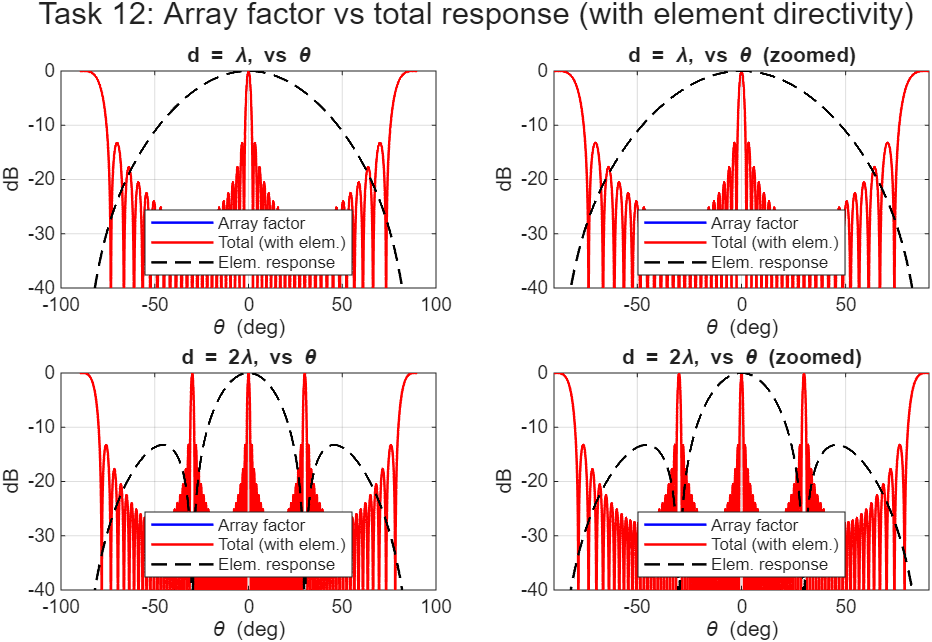
\includegraphics[width=\linewidth,height=0.52\textheight,keepaspectratio]{image-19.png}

\vspace{-0.3em}
\scriptsize
\begin{itemize}\setlength\itemsep{0pt}
  \item \textbf{$d=\lambda$:} Element response zero at $u=\pm1$ coincides with grating lobe $\Rightarrow$ suppressed at broadside. Element envelope spans full visible region.
  \item \textbf{$d=2\lambda$:} Element zeros at $u=\pm0.5,\pm1$ coincide with grating lobes $\Rightarrow$ also suppressed at broadside.
\end{itemize}
\end{frame}

% -- SLIDE: Task 13 --
\begin{frame}{Task 13 - Steering with element directivity}
\vspace{-0.3em}
\begin{columns}[T]
\column{0.48\textwidth}
\colfig{image-20.png}
\centering\scriptsize $d = \lambda$
\column{0.48\textwidth}
\colfig{Figure_14.png}
\centering\scriptsize $d = 2\lambda$
\end{columns}

\vspace{-0.3em}
\scriptsize
Steering shifts the array factor in $u$-space, but $H_e$ is \textbf{fixed} since elements dont move.

\begin{itemize}\setlength\itemsep{0pt}
  \item \textbf{$d=\lambda$:} Grating lobes shift away from element zeros and reappear. At $\theta_s=60^\circ$ a GL is partially visible but still attenuated.
  \item \textbf{$d=2\lambda$:} At $\theta_s=20^\circ$ the first GL near broadside exceeds the steered main lobe - element pattern works \emph{against} the beam. Usable scan $\lesssim 10^\circ$.
\end{itemize}

\textbf{Conclusion:} Element directivity provides excellent GL suppression at broadside but diminishes with steering. For $d>\lambda/2$ the scan range is fundamentally limited.
\end{frame}

% -- SLIDE: Code 12-13 --
\begin{frame}[fragile]{Code - Element directivity (Tasks 12-13)}
\vspace{-0.3em}
\begin{lstlisting}
% Element response for rectangular element of width d:
% H_e(kx) = sinc(kx*d/(2*pi))
elem_resp = @(d) sinc(kx * d / (2*pi));

for di = 1:2
    d = d_list(di);   % lambda, 2*lambda
    xpos = (-(M-1)/2 : (M-1)/2).' * d;
    w = ones(M,1) / M;

    W_array = beampattern(xpos, kx, w).'; % array factor (transpose to row)
    He      = elem_resp(d);               % element pattern (row)
    W_total = W_array .* He;              % total response
end

% Steering: shift kx by steering direction
for si = 1:length(steer_angles)
    theta_s = deg2rad(steer_angles(si));
    kx_steer = 2*pi/lambda * (u - sin(theta_s));
    W_steered = beampattern(xpos, kx_steer, w).' .* He;
end
\end{lstlisting}

\scriptsize Total response = array factor $\times$ element pattern. Steering shifts $W(k_x)$ but $H_e(k_x)$ stays fixed, so grating lobes reappear when steered away from broadside.
\end{frame}

% ==================================================================
\section*{Summary}
% ==================================================================

% -- SLIDE: Summary --
\begin{frame}{Summary}
\begin{enumerate}\setlength\itemsep{3pt}
  \item \textbf{Diffraction (1-2):} R-S integral reproduces near-field to far-field transition; $z_R = D^2/(4\lambda)$ for line aperture.
  \item \textbf{Grating lobes (4):} Appear for $d \ge \lambda$; $d = \lambda/2$ is the aliasing-free limit.
  \item \textbf{Kaiser window (5):} ${\sim}12$\,dB SL suppression per $1^\circ$ BW broadening; modest WNG cost.
  \item \textbf{Non-uniform spacing (6):} Case B achieves $-17.9$\,dB SL with unity weights and full WNG.
  \item \textbf{Steering (7-8):} BW increases with greater magnitude steering angle.
  \item \textbf{Thinning (9):} Preserves BW but raises SL floor; optimised placement ${\approx}5$\,dB better than random.
  \item \textbf{Element directivity (12-13):} Element response suppresses grating lobes at broadside; steering breaks the alignment.
\end{enumerate}
\end{frame}

\end{document}
